
%aika lailla tarpeeks tekstiä pitää vain lukee kunnolla läpi ja laittaa jutut oikein


Koko alusta on jaettu kahteen osaan, käyttäjäpuoli ja hallintapuoli, molemmilla on oma front- ja backend mutta ne käyttävät samaa tietokantaa.
Testailussa ja kehittämisessä tormäsin ongelmiin, kun en ollut yhdistänyt hallinta ja käyttäjäpuolta samaan tietokantaan.
%tähän väliin vielä lisää siitä miksi docker ratkaisisi tämän tai miksi valitsin dockerin
% tässä voisi kanssa olla jotain tekstiä dockedrista niin noi alemmat kappaleet ei tuu yllätyksenä.




\subsection*{Kontitus}

%kontti on sitä ja tätä
%kontin voi tehdä kontin kuvasta joka on sitä ja tätä
%kontin kuvan voi tehdä dockerfilen kautta joka on kasa ohjeita mitä suorittaa


% enemmän sanoja

Kontti on kevyt, itsenäinen ja eristetty ympäristö, joka on suuntautunut sovelluksien suorittamiseen.
Toisin kun virtuaalikoneissa, kontin mukana ei tule käyttöjärjestelmää vaan se käyttää isäntäkonetta hyödyksi, joka tekee siitä kevyemmän.
Kontti suoritetaan eristettynä prosessina ja kehittäjä voi määritellä miten kontti voi kommunikoida ulkomaailman kanssa.
\medskip

Kontit tehdään kontti kuvasta.
Kuva on binaari tilannekuva sovelluksesta, sen käytetystä softasta ja sen riippuvuuksista.
se on vahvasti määritelty ympäristö ja se ei tee oletuksia suoritus ympäristöstään, jota tekee siitä helposti siirrettävän ja skaalautuvan.
\medskip

Kontin kuvan voi tehdä Dockerfilen kautta. Dockerfile on lista ohjeita ja komentoja jotka määrittävät mitä riippuvaisuuksia, ja sovelluksia konttiin tulee.
Dockerfile on vain tekstitiedosto, joka tekee siitä myös helposti muokattavan ja jaettavan.

\medskip






\subsection*{Docker-compose}


%stack suomeksi ehk,
Docker-compose on työkalu moni kontti sovelluksille, joka mahdollistaa kontti verkon käynnistämisen, se yksinkertaistaa koko ohjelmistopinon käynnistämistä ja hallinttaa.
Docker-compose lukee docker-compose.yaml tiedostosta, miten konttia pitäisi kohdella.
Tiedostosta voi määritellä ympäristö muuttujia ja volyymejä, jolla voi määrittää voiko kontti tallentaa isäntäkoneelle tietoja.
Koko kontti verkoston voi käynnistää yhdellä "docker-compose up"{} komennolla.


\medskip


\subsection*{Testiympäristö}


Hallinta ja käyttäjä kontit saavat \verb"MONGO_URL" ympäristömuuttujan, joka on mongodb kontin osoite. Näin hallinta ja käyttäjäpoli jakaa saman tietokannan.
Molemmille on annettu volyyminä niiden lähdekoodi, joka mahdollistaa kontin päivityksen, kun teen muutosta koodipohjaan.
\medbreak

\medskip

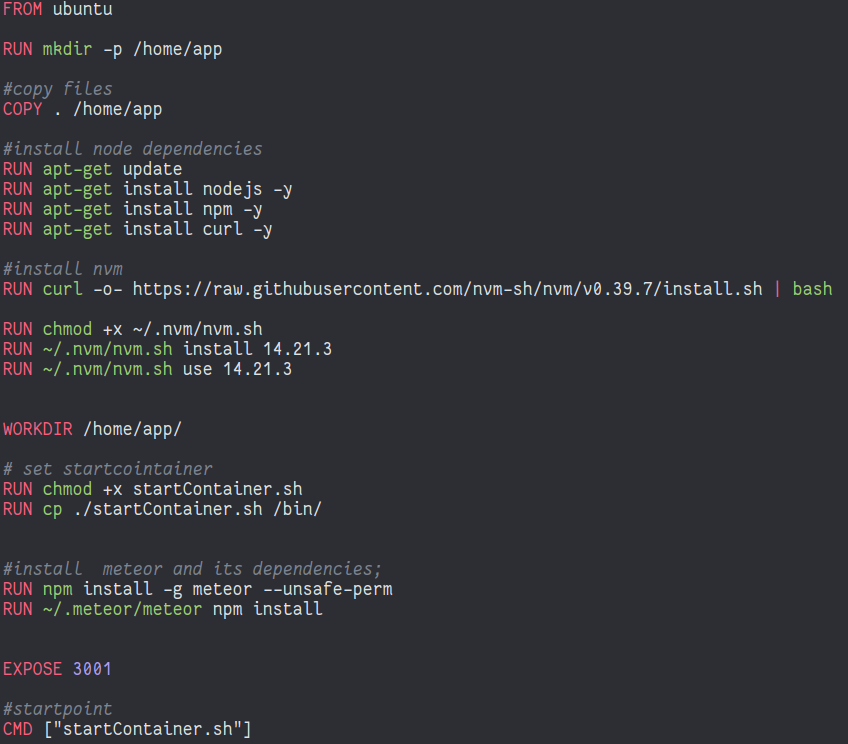
\includegraphics[height=10cm]{src/public/dockerfile.png} \\
Hallinta puolen dockerfile.
\medskip

Hallinta ja käyttäjä puolen Docker kuvat ovat pohjautuvat molemmat ubuntu lts ja ovat muuten identtisiä porttia lukuun ottamatta.
Kuvassa ensimmäiseksi ladataan uudet päivitykset, jonka jälkeen ladataan nodejs ja siitä 14.21.3 versio, jota projekti käyttää.
Sitten ladataan meteor, jonka jälkeen käynnistetään "startcontainer"{} scripti.
\medskip

startcontainer scripti on seuraava. 
\medskip
\begin{tcolorbox}
~/.meteor/meteor --allow-incompatible-update --settings ./settings-development.json --allow-superuser --port 3001
\end{tcolorbox}

Startcontainer scripti on yksi shell komento ja on muuten identtinen hallinta ja käyttäjä puolella paitsi hallinnalla portti on 3001 ja käyttäjällä 3002.
Skripti käynnistää meteorin ja ohjaa sitä käyttämään settings-development.json tiedostoa, jossa on ympäristömuuttujia kuten AWS avaimet.
Settings-development.json tiedosto ei tule kontin kuvaan mukaan vaan se annetaan erikseen volyymin mukana docker-composen kautta.
\medskip

mongodb:llä oli oma docker kuva, jonka pystyi ladata docker hubista, dockerin verkko palvelimelta, johon voi tallentaa docker kuvia, joten se ei tarvinnut omaa dockerfileä.
\medskip


\subsection*{Yhteenveto}

Sain docker-composen avulla tehtyä kontti verkon, jossa hallinta ja käyttäjä puoli toimii erikseen mutta kommunikoi saman tietokannan kanssa 
Koko sovellus on nyt helpommin käynnistettävissä ja siirrettävissä.
Dockeria käyttäen voisi myös ladata suoraan oikean python version, jolloin koodin ensimmäistä latausta varten ei tarvitse asettaa omaa python virtuaali ympäristöä. 
Mutta tätä en tehnyt sillä annoin kontille jo valmiiksi asennetun projektin.
